\documentclass[border=4pt]{standalone}
% Shared by the independently buildable vector figures.
\usepackage[T1]{fontenc}
\usepackage{amsmath,amssymb,newpxtext,newpxmath}
\usepackage[semibold]{sourcesans}
\usepackage{pgfplots}
\pgfplotsset{compat=1.18}
\usetikzlibrary{arrows.meta,calc,positioning}
\usepgfplotslibrary{groupplots}
\definecolor{ink}{HTML}{19303A}
\definecolor{sea}{HTML}{00675E}
\definecolor{clay}{HTML}{A24725}
\definecolor{muted}{HTML}{4C636C}
\definecolor{rulegray}{HTML}{CAD4D4}
\definecolor{wash}{HTML}{EAF4F0}
\definecolor{warm}{HTML}{F7EEE5}
\color{ink}
\tikzset{every picture/.style={font=\sffamily\small},
  arrow/.style={-{Stealth[length=2mm]},line width=.8pt,draw=muted}}
\pgfplotsset{companion/.style={axis lines=left,axis line style={draw=muted},
  tick style={draw=muted},ticklabel style={font=\sffamily\footnotesize,text=muted},
  label style={font=\sffamily\small},grid=major,grid style={draw=rulegray!64,line width=.25pt},
  tick align=outside,enlarge x limits=false,scaled ticks=false,
  every axis plot/.append style={line join=round},
  legend style={draw=none,fill=none,font=\sffamily\footnotesize},
  title style={font=\sffamily\bfseries\small,anchor=south west,at={(0,1.03)}}}}

\begin{document}
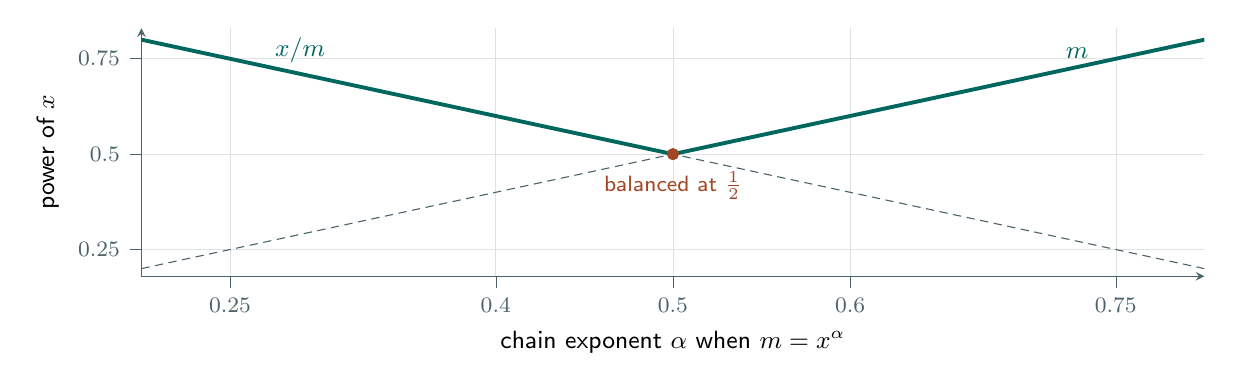
\begin{tikzpicture}
\begin{axis}[companion,width=13.5cm,height=3.15cm,scale only axis,
  xmin=.2,xmax=.8,ymin=.18,ymax=.83,xtick={.25,.4,.5,.6,.75},ytick={.25,.5,.75},
  xlabel={chain exponent $\alpha$ when $m=x^\alpha$},ylabel={power of $x$}]
\addplot[sea,line width=1.4pt] coordinates {(.2,.8)(.5,.5)(.8,.8)};
\addplot[muted,densely dashed] coordinates {(.2,.2)(.5,.5)(.8,.2)};
\addplot[only marks,mark=*,mark size=2pt,color=clay] coordinates {(.5,.5)};
\node[anchor=south west,font=\sffamily\small,text=sea] at (axis cs:.27,.715){$x/m$};
\node[anchor=south east,font=\sffamily\small,text=sea] at (axis cs:.74,.725){$m$};
\node[anchor=north,font=\sffamily\footnotesize,text=clay] at (axis cs:.5,.48){balanced at $\tfrac12$};
\end{axis}
\end{tikzpicture}
\end{document}
